\documentclass[handout,aspectratio=169,11pt,xcolor={dvipsnames},hyperref={pdftex,pdfpagemode=UseNone,hidelinks,pdfdisplaydoctitle=true},usepdftitle=false]{beamer}
%----------------------------------------------------------------------
% Preamble
%----------------------------------------------------------------------

\usepackage{amsmath}
\usepackage{presentation}
\usepackage{tikz}
\usetikzlibrary{arrows.meta, positioning, calc, decorations.pathreplacing, fit,
backgrounds}
\usepackage{mathrsfs}

%----------------------------------------------------------------------
% Title information
%----------------------------------------------------------------------

\title{Measuring Macroeconomic and Financial Uncertainty: Impact for the Mexican Economic Growth Expectation}
\information{Jesus Lopez-Perez}{The Graduate Center, CUNY}
\date{May 15, 2026}

%----------------------------------------------------------------------
% Document
%----------------------------------------------------------------------

\begin{document}

%------ Title slide ----------------------------------------------------

\begin{frame}
\titlepage
 \end{frame}

%======================================================================
\section{Motivation}
%======================================================================
\begin{frame}{Uncertainty in macroeconomics}


\textbf{Greenspan (2003):} ``Uncertainty is not just an important feature of the monetary policy landscape; it is the defining characteristic of that landscape''

\vspace{4mm}

Some concepts of uncertainty in the literature: 
\begin{itemize}

\item \textbf{EPU} - (Baker, Bloom and Davis) How uncertainty is the Policy Environment that households and firms face.
\item \textbf{VIX} - How much financial markets expect asset prices to fluctuate.
\item \textbf{JLN} - (Jurado, Ludvigson and Ng) How unpredictable in macroeconomy.
\item \textbf{LMN} - (Ludvigson, Ma and Ng) What are the roles of \textbf{macroeconomic} and \textbf{financial} uncertainty.
\end{itemize}



\end{frame}


\begin{frame}{Why is this important?}
Effects of heightened uncertainty
\begin{itemize}
\item More dispersion and negative skewed future growth distribution of economic activity
\item Non-linear and asymmetric responses to uncertainty
\item Higher asset prices volatility
\end{itemize}

Remark:
Monetary policy makers should conducts a balance of risks weighing downside risks ---shocks to production, short and long term unemployment--- and upside risks---inflation, to determine the entire probability distribution of expected economic growth. 


In this context Adrian, Boyarchenko and Gianone (2019), propose a methodology to determine \textit{what is the worst GDP outcome that we should expect with given probability?}

\end{frame}

%------------------------------------------------

\begin{frame}{Literature review -- for the Mexican economy}
\begin{itemize}
\item Salgado and Trujillo (2025). How macroeconomic uncertainty, using the Financial Conditions Index (Carrillo and Garcia, 2021), affects growth expectations.
\item  Catal\'an (2019) How uncertainty shocks from EPU affect prices (interest rates, wages) and, consequently, economic activity (investment and employment).
\item  Cebreros (2000) How trade policy uncertainty affects FDI.

\end{itemize}
\end{frame}

\begin{frame}{Research question}
\begin{itemize}
\item \textbf{What role does macroeconomic and financial uncertainty play in the determination of growth expectation for the Mexican economy?}

\item \textbf{Contribution:} disentangle the MU from FU and apply the GaR methodology.

\end{itemize}

\end{frame}

\section{Methodology}
\begin{frame}{Methodology}
\begin{enumerate}
\item Estimate common trends to the Mexican economy, following the work by Corona et al (2021). They develop a panel of 26 variables that are used to nowcast Mexican monthly economic activity indicator (IGAE).
\item Compute \textit{macro} uncertainty, MU, and \textit{financial} uncertainty, FU, indicators, following Ludvignson, Ma and Ng (2021), as the unforeseeable component of economic variables after extracting all common predictable variation in the DFM.
\item Estimate a SVAR to identify causal direction between MU, FU and economic activity. 
\item Estimating the entire conditional distribution of growth for evaluating uncertainty’s impact in the Mexican economy (Adrian, Boyarchenko and Gianone, 2019).
\end{enumerate}
\end{frame}

%\begin{frame}{Model}
%\begin{itemize}
%
%
%\item GARCH(1,1) on $e_{it}$ $\Rightarrow$ $\sigma_{it}$, then aggregate:
%\[
%MU_t = \mathrm{mean}\lbrace\sigma_{it} : i \in \mathrm{Macro}\rbrace, \quad
%FU_t = \mathrm{mean}\lbrace\sigma_{it} : i \in \mathrm{Financial}\rbrace
%\]
%
%\item SVAR: $X_t = (MU_t,\, IGAE_t,\, FU_t)'$
%\begin{itemize}
%\item Ordering A: $MU \to IGAE \to FU$ \quad (LMN baseline)
%\item Ordering B: $FU \to IGAE \to MU$ \quad (robustness)
%\end{itemize}
%
%\end{itemize}
%\end{frame}

\section{Data}


\begin{frame}{Mexican Economic Activity Indicator}
\begin{figure}
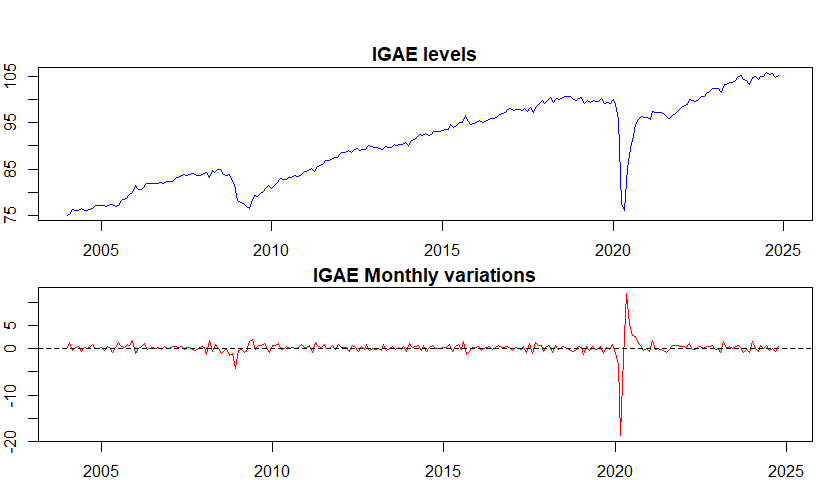
\includegraphics[width=.8\textwidth]{../ioae_assesment/outputs/lmn/IGAE.png}
\end{figure}
\end{frame}

\begin{frame}{Unit root tests}
\begin{columns}[T]
\begin{column}{0.62\textwidth}
\small
\begin{tabular}{llrrrr}
\hline
\textbf{Series} & \textbf{Test} & \textbf{Stat} & \textbf{CV 1\%} & \textbf{CV 5\%} & \textbf{CV 10\%} \\
\hline
\multicolumn{6}{l}{\textit{ADF — H$_0$: unit root; reject if stat $<$ CV}} \\
\hline
Levels           & ADF &  $-4.792$ & $-3.980$ & $-3.420$ & $-3.130$ \\
Monthly var.     & ADF & $-13.030$ & $-3.460$ & $-2.880$ & $-2.570$ \\
\hline
\multicolumn{6}{l}{\textit{PP — H$_0$: unit root; reject if stat $<$ CV}} \\
\hline
Levels           & PP  &  $-3.761$ & $-3.998$ & $-3.429$ & $-3.138$ \\
Monthly var.     & PP  & $-11.934$ & $-3.458$ & $-2.873$ & $-2.573$ \\
\hline
\multicolumn{6}{l}{\textit{KPSS — H$_0$: stationary; reject if stat $>$ CV}} \\
\hline
Levels           & KPSS &  $0.203$ &  $0.216$ &  $0.176$ &  $0.146$ \\
Monthly var.     & KPSS &  $0.022$ &  $0.739$ &  $0.574$ &  $0.463$ \\
\hline
\end{tabular}
\end{column}

\begin{column}{0.35\textwidth}


For levels evidence is mixed — ADF/PP reject the unit root at 5\% but KPSS also rejects stationarity at 5\%.

\vspace{2mm}


Monthly variation is $I(0)$: ADF and PP reject the unit root, and KPSS does not reject stationarity at any conventional level.


\vspace{2mm}

This validates using IGAE monthly growth rate in the VAR.

\end{column}
\end{columns}
\end{frame}


\begin{frame}{Structural breaks at Mexican recession dates}

\begin{columns}[T]

\begin{column}{0.45\textwidth}
\small
\begin{tabular}{llrr}
\hline
\textbf{Series} & \textbf{Date} & \textbf{F} & \textbf{p-val} \\
\hline
\multicolumn{4}{l}{\textit{IGAE levels}} \\
\hline
Levels & 2009/05 & \textcolor{black}{243.86} & \textcolor{black}{0.000} \\
Levels & 2020/05 & \textcolor{black}{115.32} & \textcolor{black}{0.000} \\
\hline
\multicolumn{4}{l}{\textit{IGAE monthly variation}} \\
\hline
Monthly var. & 2009/05 & 0.271 & 0.603 \\
Monthly var. & 2020/05 & 1.657 & 0.199 \\
\hline
\multicolumn{4}{l}{\footnotesize Chow test, H$_0$: no structural break.} \\
\multicolumn{4}{l}{\footnotesize Dates: CEEY recession chronology.} \\
\end{tabular}
\end{column}

\begin{column}{0.52\textwidth}
Structural breaks are present in the \textit{level} of IGAE but \textbf{not} in its monthly growth rate.

\vspace{3mm}

\begin{itemize}
\item The 2009 and 2020 recessions produced \textbf{permanent level shifts} in economic activity.

\vspace{2mm}

\item Monthly variation does not reflect this shifts is \textbf{structurally stable} across both episodes ($p > 0.10$).

\vspace{2mm}

\item First-differencing simultaneously removes the unit root and the structural breaks.


\end{itemize}
\end{column}

\end{columns}
\end{frame}


\begin{frame}{Endogenous structural breaks — IGAE}

\begin{columns}[T]

\begin{column}{0.52\textwidth}
\small\textbf{Bai-Perron (BIC-optimal partition)}

\vspace{2mm}
\small
\begin{tabular}{lcc}
\hline
 & \textbf{Levels} & \textbf{Monthly var.} \\
\hline
Optimal breaks ($m$) & 6 & 0 \\
BIC & 1234 & 963.7 \\
\hline
\end{tabular}

\vspace{3mm}
\textit{Levels} — break dates ($m = 6$):

\vspace{1mm}
\begin{tabular}{ll}
\hline
\textbf{Date} & \textbf{Episode} \\
\hline
2006/01 & Post-NAFTA adjustment \\
2011/05 & Euro-area sovereign crisis \\
2014/03 & Oil price decline \\
2016/08 & US electoral uncertainty \\
\textcolor{black}{2020/02} & \textcolor{black}{COVID-19 recession} \\
2022/03 & Post-pandemic inflation surge \\
\hline
\end{tabular}

\vspace{3mm}
\textit{Monthly variation} — no breaks detected. \\
{\tiny BIC strictly decreasing from $m=0$; \texttt{breakpoints()} returns NA.}

\end{column}

\begin{column}{0.45\textwidth}
\small\textbf{Zivot-Andrews }

\vspace{2mm}
\small
\begin{tabular}{lrrl}
\hline
\textbf{Series} & \textbf{Stat} & \textbf{CV 1\%} & \textbf{Break} \\
\hline
Levels       & $-5.697$ & $-5.57$ & 2020/02 \\
Monthly var. & $-12.797$ & $-5.34$ & 2020/04 \\
\hline
\multicolumn{4}{l}{Both reject unit root at 1\%.} \\
\end{tabular}


\small
\begin{itemize}

\item Bai-Perron identifies \textbf{six level shifts} in IGAE, concentrated around macro events. 

\vspace{1mm}

\item Monthly growth rate shows \textbf{no structural breaks} — the BIC selects $m = 0$. 

\vspace{1mm}

\item Zivot-Andrews confirms break at ($-5.70 < -5.57$) and rejects the unit root for monthly variation ($-12.80 \ll -5.34$).

\vspace{1.5mm}

\end{itemize}

\end{column}
\end{columns}
\end{frame}


\begin{frame}{Data for DFM}
The panel time series consists of 26 variables with the following characteristics:
\begin{itemize}
\item Monthly frequency, 
\item Starting from January 2004, with some available through January 2025. 
\item All variables have been obtained in seasonally adjusted form; if not, they have been adjusted using the X-13ARIMA-SEATS method. This seasonal adjustment relies on the automatic modeling procedure implemented in the seas function from R’s seasonal package. 
\item Optimal transformation is applied  first-differences, monthly variation, yearly variation such that it maximize the correlation with IGAE.
\end{itemize}

\end{frame}

\begin{frame}{Data: variable panel}
\vspace{-1mm}
\begin{columns}[T]

%--- Left column: macro 1-14 ---
\begin{column}{0.50\textwidth}
\tiny
\begin{tabular}{p{1.5cm}p{2.6cm}l}
\hline
\textbf{Variable} & \textbf{Description} & \textbf{Trans.} \\
\hline
\multicolumn{3}{l}{\textit{Macro variables}} \\
\hline
IMAI             & Industrial production          & monthly \\
Sales            & Retail sales                   & monthly \\
U                & Unemployment                   & monthly \\
M                & Imports                        & monthly \\
Conf Constr      & Construction confidence        & monthly \\
Conf Manuf       & Manufacturing confidence       & monthly \\
Conf Trade 		& Trade confidence  & monthly \\
Conf Serv        & Services confidence            & monthly \\
Trend L Manuf    & Manuf.\ employment trend       & monthly \\
Industrial USA   & U.S.\ industrial production    & monthly \\
ANTAD            & ANTAD retail sales             & monthly \\
Automotive       & Vehicle production             & monthly \\
Hotel            & Hotel occupancy                & linear  \\
Gas              & Gasoline sales                 & monthly \\
\hline
\end{tabular}
\end{column}

%--- Right column: macro 15-21 + financial ---
\begin{column}{0.50\textwidth}
\tiny
\begin{tabular}{p{1.5cm}p{2.6cm}l}
\hline
\textbf{Variable} & \textbf{Description} & \textbf{Trans.} \\
\hline
\multicolumn{3}{l}{\textit{Macro variables (cont.)}} \\
\hline
IMSS             & IMSS formal employment         & monthly \\
Remittances      & Remittances inflows            & monthly \\
X                & Exports                        & monthly \\
PMI              & Manufacturing orders           & monthly \\
U USA            & U.S.\ unemployment rate        & monthly \\
Manuf USA        & U.S.\ manufacturing activity   & monthly \\
PIBO             & Timely GDP estimate (INEGI)    & monthly \\
\hline
\multicolumn{3}{l}{\textit{Financial variables}} \\
\hline
IPC              & Stock exchange index           & annual  \\
E                & Exchange rate                  & monthly \\
IR 28            & Short-term interest rate       & annual  \\
SP 500           & S\&P 500 Index                 & annual  \\
Cards            & Credit/debit card transactions & monthly \\
SPEI             & Interbank electronic transfers & monthly \\
\hline
\end{tabular}
\end{column}

\end{columns}
\vspace{1mm}
{\tiny
Trans.: transformation applied to maximise correlation with IGAE growth.
All series seasonally adjusted via X-13ARIMA-SEATS.
}
\end{frame}




\begin{frame}{Macroeconomic variables panel }
\begin{figure}
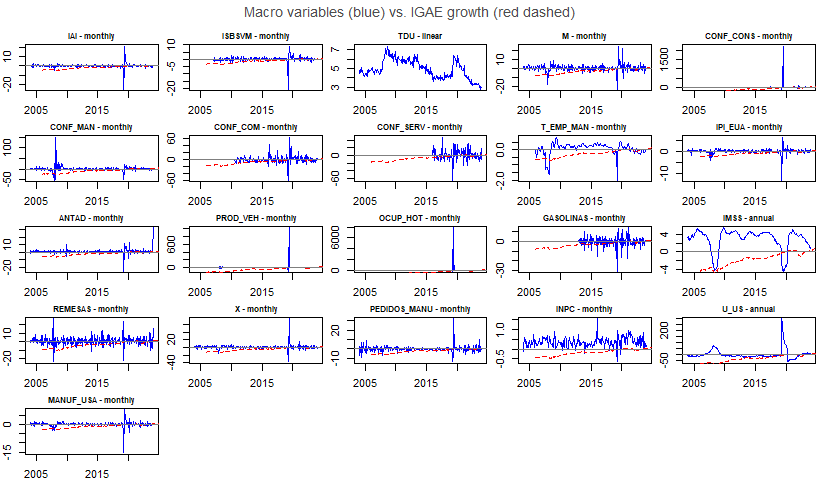
\includegraphics[width=\textwidth]{../ioae_assesment/outputs/lmn/macro_vars.png}
\end{figure}
\end{frame}


\begin{frame}{Financial variables panel }
\begin{figure}
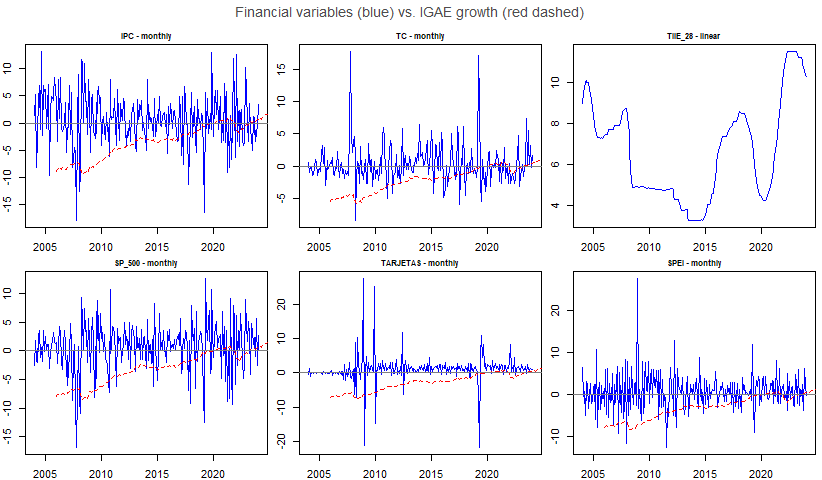
\includegraphics[width=.8\textwidth]{../ioae_assesment/outputs/lmn/fin_vars.png}
\end{figure}
\end{frame}

\section{DFM extraction}

\begin{frame}{DFM}
\begin{itemize}

\item Formally, let $\mathbf{X}_t$ be the set of data, estimate the DFM:
\[
\mathbf{X}_t=\mathbf{P} \mathbf{F}_t + \boldsymbol{\varepsilon}_t
\]

\item Idiosyncratic component: $e_{it} = x_{it} - F_t'\lambda_i$
\end{itemize}
\end{frame}

\begin{frame}{Determining the number of factors Bai \& Ng (2002) IC}

\begin{columns}[T]

\begin{column}{0.48\textwidth}
\small
\begin{tabular}{crrrr}
\hline
$r$ & \textbf{IC1} & \textbf{IC2} & \textbf{IC3} \\
\hline
0 & $-0.004$ & $-0.004$ & $-0.004$ \\
1 & $-0.191$ & $-0.186$ & $-0.200$ \\
2 & $-0.200$ & $-0.192$ & $-0.219$ \\
3 & $-0.205$ & $-0.192$ & $-0.233$ \\
4 & $-0.208$ & $-0.190$ & $-0.245$ \\
5 & $-0.215$ & $-0.193$ & $-0.262$ \\
6 & $-0.218$ & $-0.192$ & $-0.274$ \\
\textbf{7} & $\mathbf{-0.233}$ & $\mathbf{-0.202}$ & $-0.298$ \\
\textbf{8} & $-0.228$ & $-0.193$ & $\mathbf{-0.302}$ \\
\hline
\end{tabular}


\end{column}

\begin{column}{0.50\textwidth}

IC1 and IC2 select $r = 7$. IC3 suggests $r = 8$.

\vspace{4mm}

\begin{itemize}

  \item Seven factors explain \textbf{66.9\%} of total panel variance.

  \vspace{1mm}

  \item The remaining \textbf{33.1\%} is idiosyncratic variance — to be used for the GARCH. 

\end{itemize}

\end{column}
\end{columns}
\end{frame}

\begin{frame}
\begin{figure}
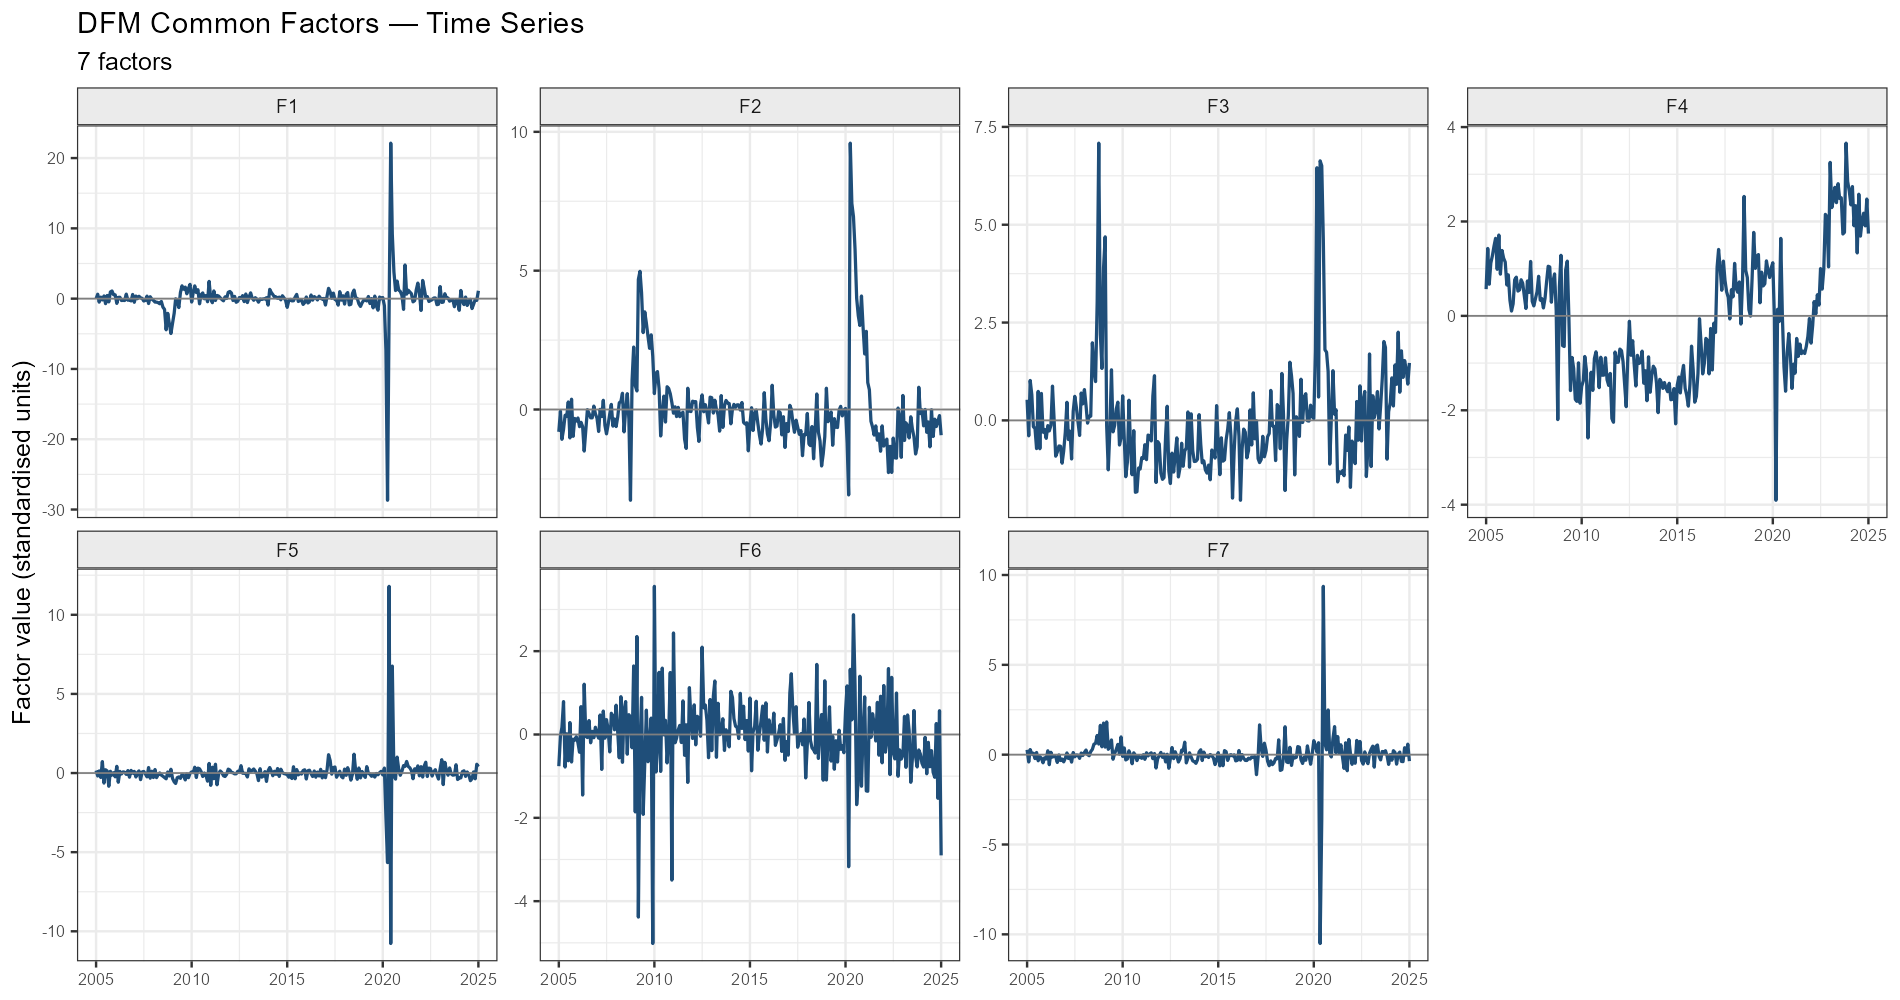
\includegraphics[scale=.6]{../ioae_assesment/outputs/lmn/fig7_factors_ts.png}
\end{figure}
\end{frame}


\section{Uncertainty extraction}

\begin{frame}{Uncertainty extraction — GARCH(1,1) on idiosyncratic components}

\begin{enumerate}

\item[Step 1] — Idiosyncratic residual

After the DFM, the idiosyncratic component for variable $i$ at time $t$ is: $e_{it} = x_{it} - \mathbf{F}_t'\boldsymbol{\lambda}_i$
$e_{it}$.

\item[Step 2] — GARCH(1,1) per variable

For each variable $i$, fit: $e_{it} = \sigma_{it}\,\eta_{it}, \qquad \eta_{it} \sim \mathit{iid}(0,1)$
\[
\sigma^2_{it} = \omega_i + \alpha_i\,e^2_{i,t-1} + \beta_i\,\sigma^2_{i,t-1}
\]
%with $\omega_i > 0$,\ $\alpha_i, \beta_i \geq 0$,\ $\alpha_i + \beta_i < 1$.


$\sigma_{it}$ is the \textbf{conditional standard deviation} of the unforeseeable component (JLN measure of uncertainty).


\item[Step 3] — Aggregate into MU and FU

$MU_t = \frac{1}{N_{{M}}}\sum_{i \in {M}} \sigma_{it}, \quad$
$FU_t = \frac{1}{N_{{F}}}\sum_{i \in {F}} \sigma_{it}$

Both indices are standardised to zero mean and unit variance.

\end{enumerate}

\end{frame}


\begin{frame}
\begin{figure}
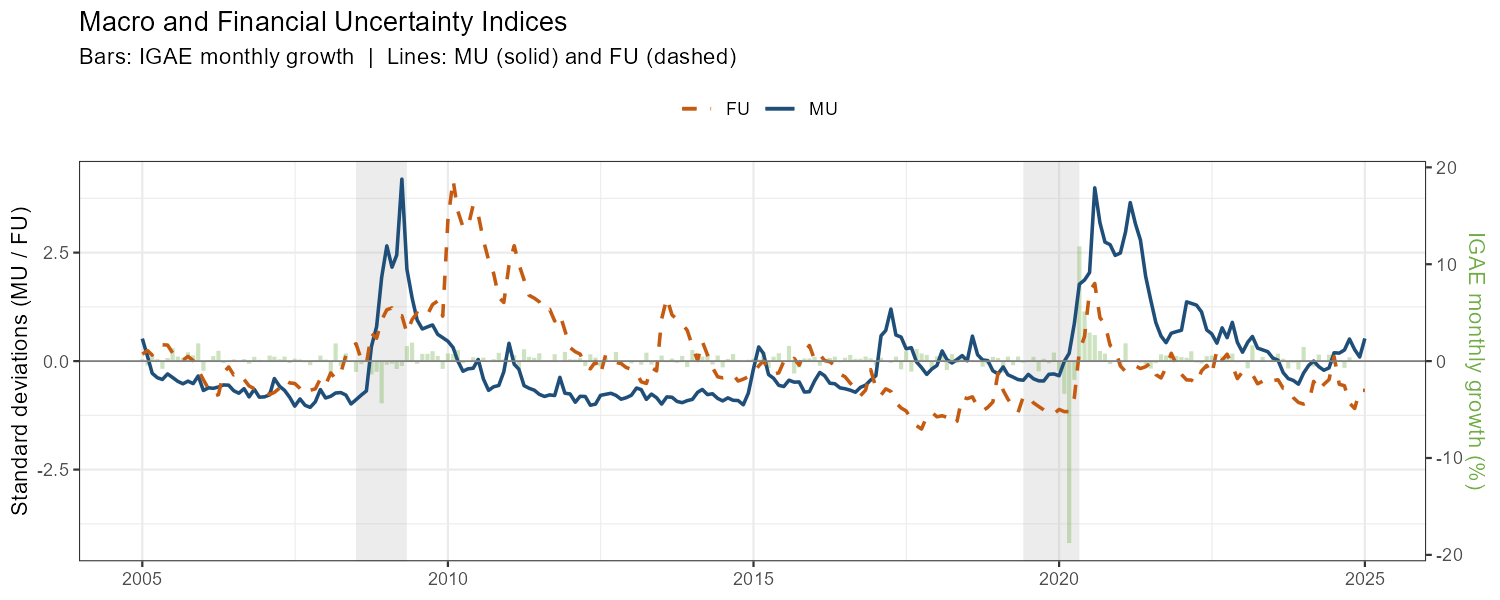
\includegraphics[scale=.55]{../ioae_assesment/outputs/lmn/fig1_mu_fu_indices.png}
\end{figure}
\end{frame}



\begin{frame}
\begin{figure}
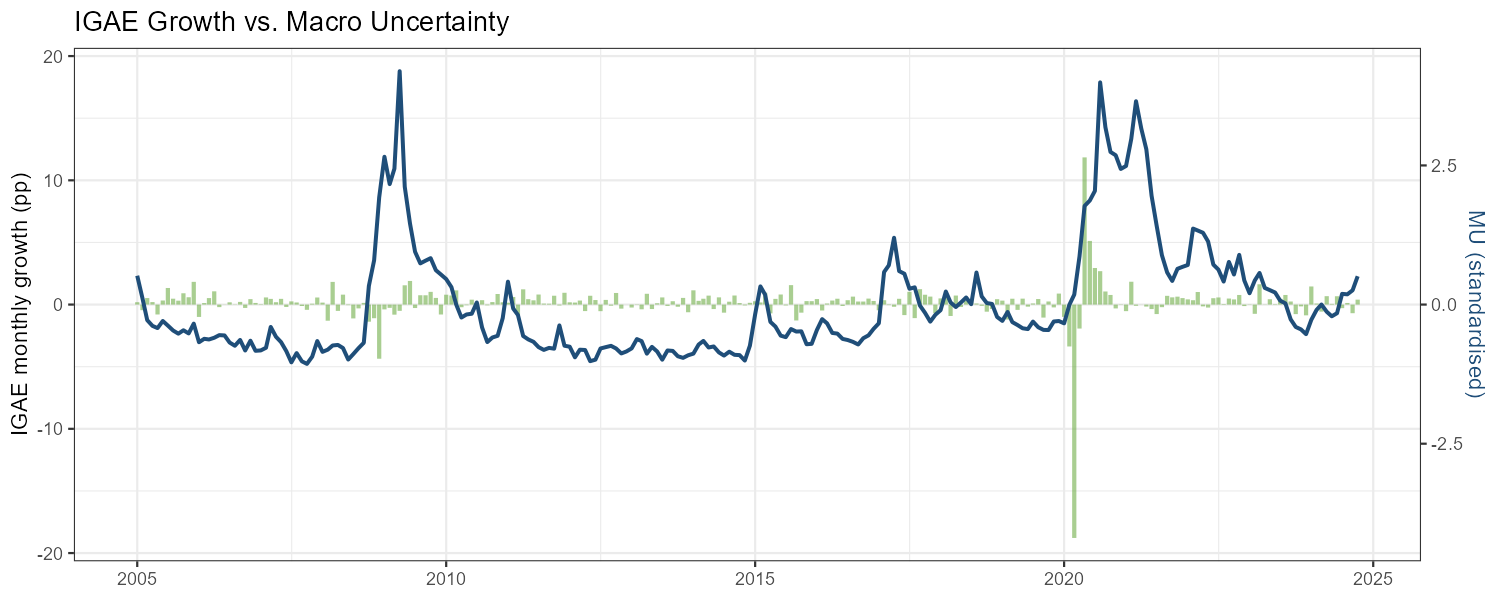
\includegraphics[scale=.55]{../ioae_assesment/outputs/lmn/fig3_igae_vs_mu.png}
\end{figure}
\end{frame}

\section{SVAR}
\begin{frame}{VAR lag selection criteria}

\begin{columns}[T]

\begin{column}{0.50\textwidth}

\textbf{Model}
\[
\mathbf{X}_t = \begin{pmatrix} MU_t \\ IGAE_t \\ FU_t \end{pmatrix}, \qquad
\]

\[
\mathbf{X}_t = \mathbf{c} + \sum_{j=1}^{p} \mathbf{A}_j \mathbf{X}_{t-j} + \mathbf{u}_t
\]





\end{column}

\begin{column}{0.47\textwidth}
\small\textbf{Information criteria ($p_{\max} = 6$)}

\vspace{1mm}
\small
\begin{tabular}{cccc}
\hline
$p$ & \textbf{AIC} & \textbf{HQ} & \textbf{SC}  \\
\hline
1 & $-3.42$ & $-3.35$ & $\mathbf{-3.24}$  \\
2 & $-3.48$ & $\mathbf{-3.36}$ & $-3.17$  \\
3 & $-3.44$ & $-3.26$ & $-2.99$  \\
4 & $\mathbf{-3.51}$ & $-3.28$ & $-2.93$  \\
5 & $-3.50$ & $-3.21$ & $-2.78$  \\
6 & $-3.47$ & $-3.12$ & $-2.62$  \\
\hline
\end{tabular}

\begin{itemize}

  \item SC selects $p = 1$; HQ selects $p = 2$; AIC selects $p = 4$.
       

  \vspace{2mm}


  \item With $p = 1$ and $K = 3$ variables the VAR has
        $K \times (K + 1) = 12$ free parameters.
\item Choose 1 lag. 
\end{itemize}

\end{column}
\end{columns}


\end{frame}


\begin{frame}{IRF}
\begin{figure}
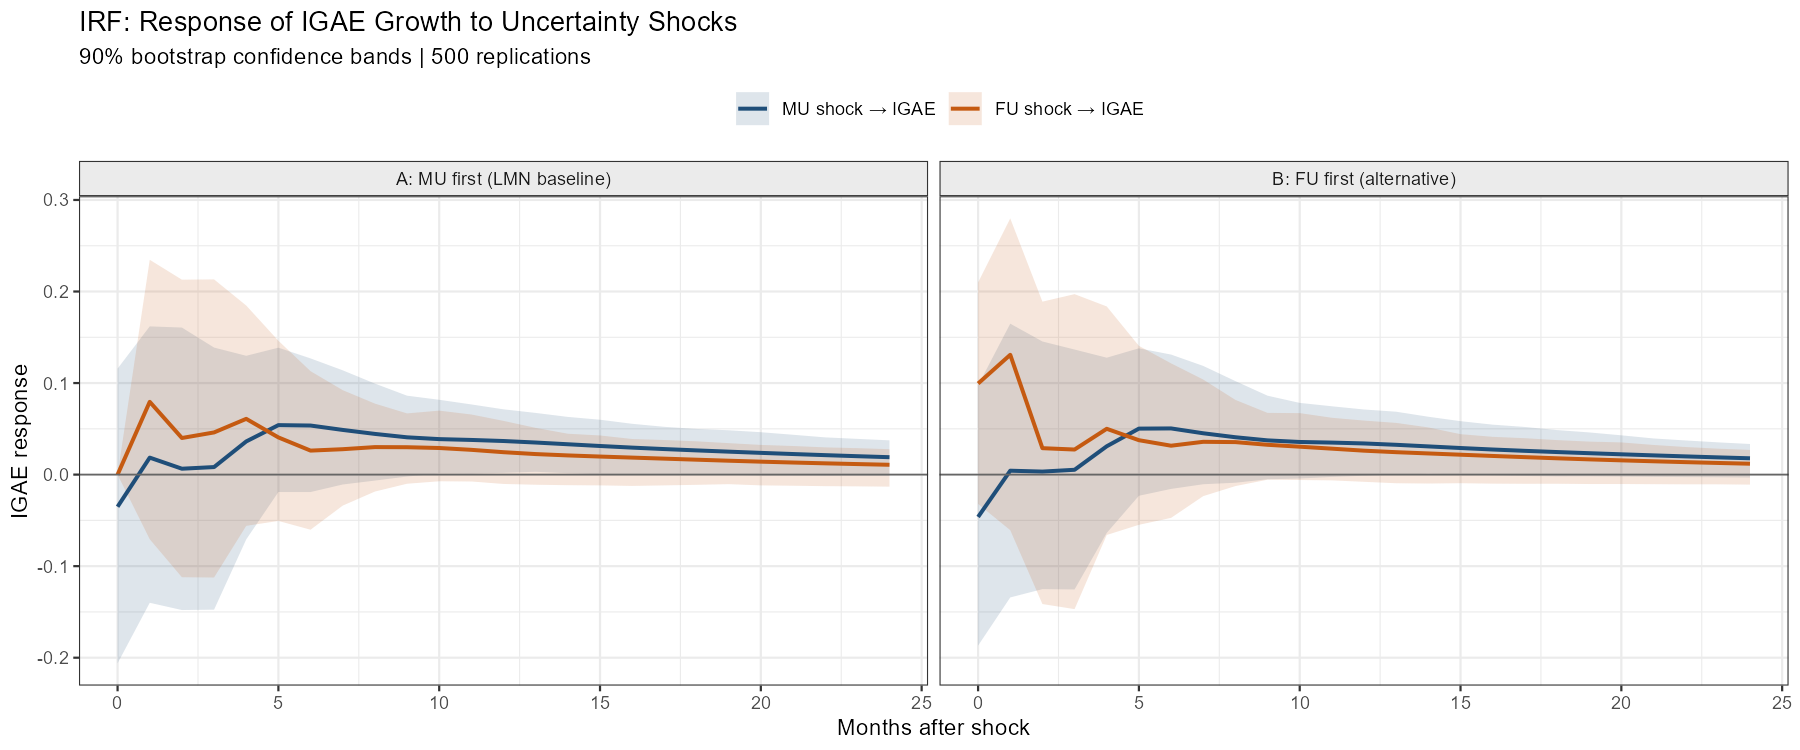
\includegraphics[scale=.5]{../ioae_assesment/outputs/lmn/fig4_irfs.png}
\end{figure}
\end{frame}



\begin{frame}{FEVD}
\begin{figure}
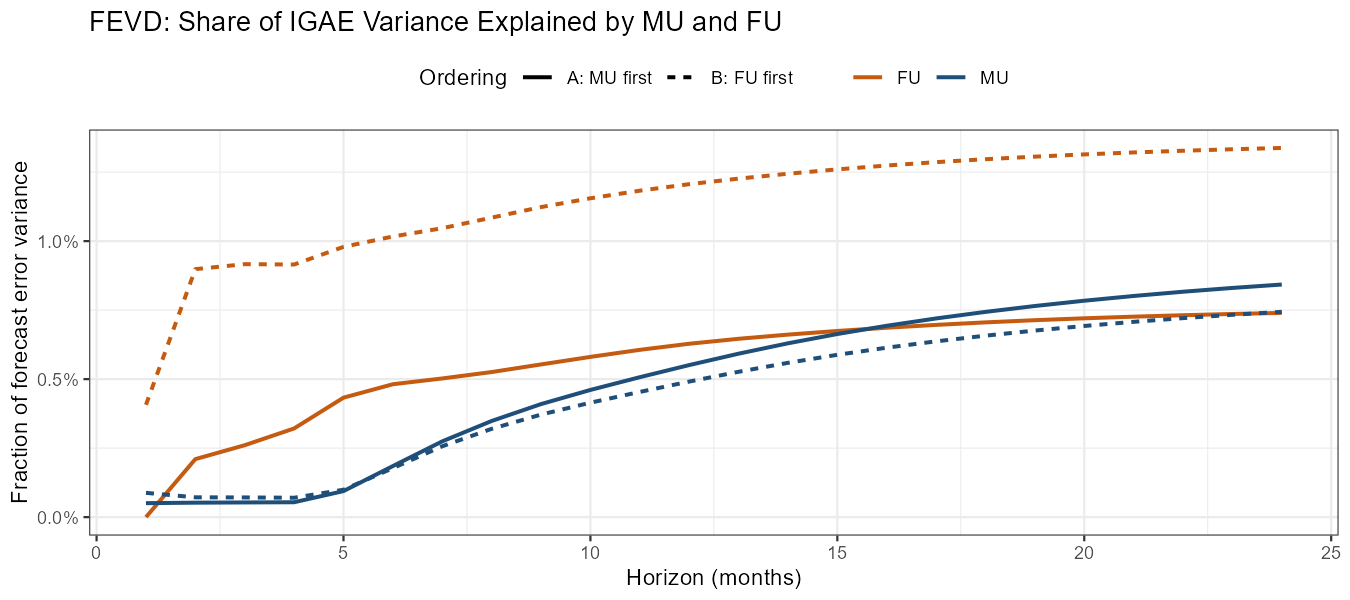
\includegraphics[scale=.55]{../ioae_assesment/outputs/lmn/fig5_fevd.png}
\end{figure}
\end{frame}


\begin{frame}{IRF with LP}
\begin{figure}
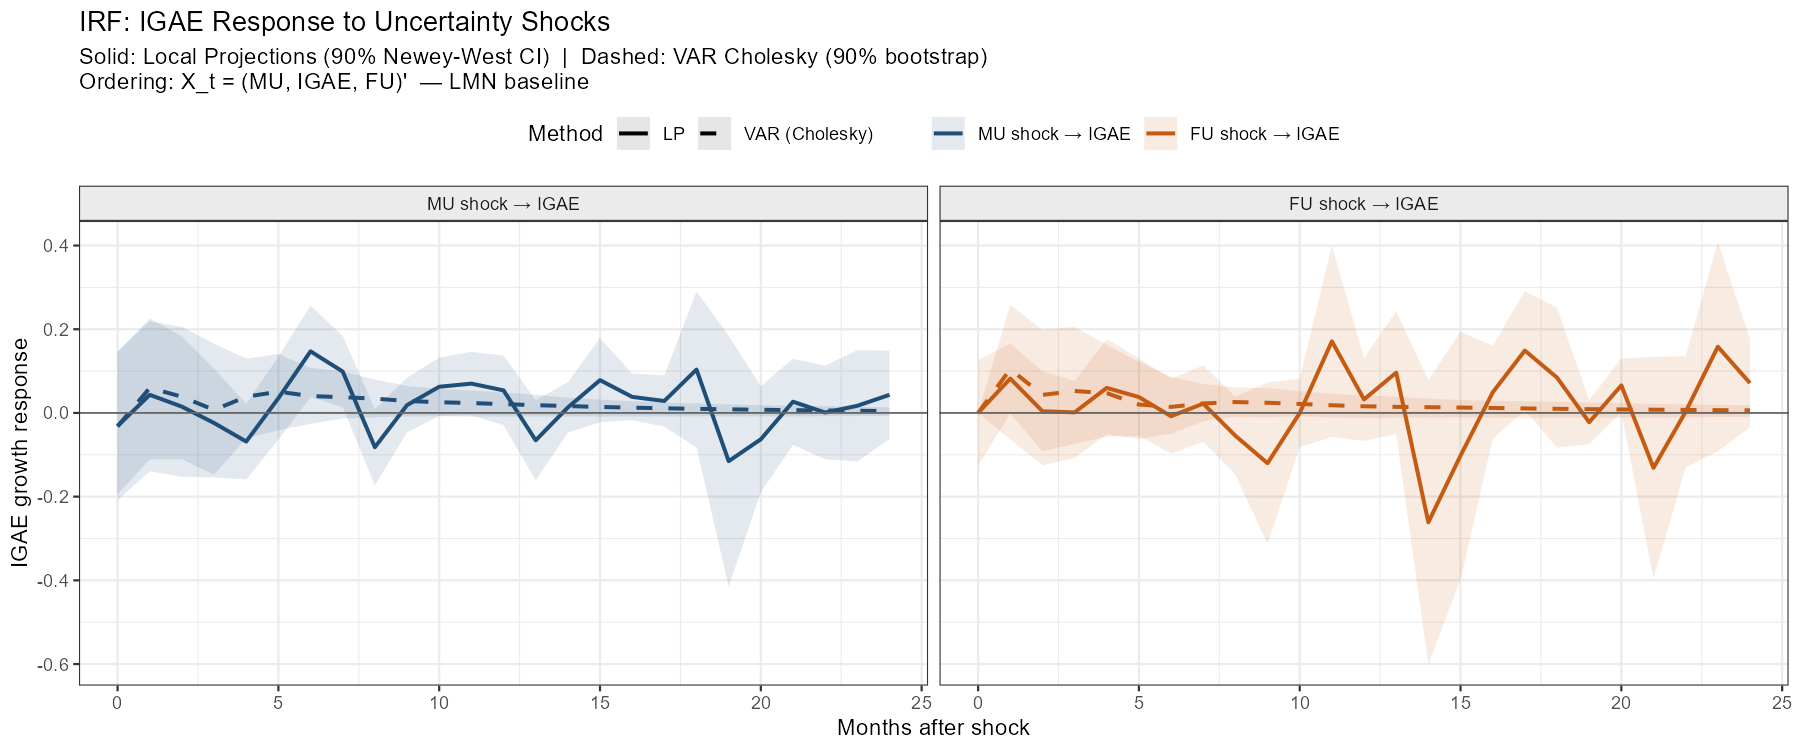
\includegraphics[scale=.5]{../ioae_assesment/outputs/lmn/fig6_lp_irf.png}
\end{figure}
\end{frame}

\section{Conclusions}
\begin{frame}{Main takeaways}
\begin{itemize}
\item DFM is a powerful tool applicable for many purposes: index construction, nowcasting, uncertainty.
\item The methodology of JLN/LMN is useful for measurement of unobserved variables: uncertainty.
\item SVAR provides a framework to identify causal relations in these variables.
\end{itemize}
\end{frame}


\begin{frame}{Next steps}
\begin{itemize}
\item Perform the GaR methodology (Adrian, et al. 2019)
\item Perform Cyclical + Permanent decomposition
\item Elaborate cointegration analysis with the variables in levels
\item Compare the results with those from Salgado and Trujillo (2025)
\end{itemize}
\end{frame}

\begin{frame}{References}
Adrian, T., Boyarchenko, N., \& Giannone, D. (2019).
Vulnerable Growth.
\textit{American Economic Review}, 109(4), 1263--1289.

Jurado, K., Ludvigson, S. C., \& Ng, S. (2015).
Measuring Uncertainty.
\textit{American Economic Review}, 105(3), 1177--1216.

Ludvigson, S. C., Ma, S., \& Ng, S. (2021).
Uncertainty and Business Cycles: Exogenous Impulse or Endogenous Response?
\textit{American Economic Journal: Macroeconomics}, 13(4), 369--410.

Corona, F., Gonzalez-Farias, G., and Lopez-Perez, J.. (2021). A nowcasting approach to generate timely estimates of Mexican economic activity: An application to the period of COVID-19.  

\end{frame}

\end{document}
